\documentclass{article}

\usepackage[utf8]{inputenc}
\usepackage[T1]{fontenc}
\usepackage{hyperref}
\usepackage{url}
\usepackage{booktabs}
\usepackage{amsfonts}
\usepackage{nicefrac}
\usepackage{microtype}
\usepackage{nips_2017}
\usepackage{graphicx}
\usepackage{subcaption}
\usepackage{amsmath}
\usepackage{natbib}

\setcitestyle{numbers,open={[},close={]}}
\graphicspath{ {./images/} }

\title{Deep Multimodal Generative Models for Weakly-Supervised Learning}

\author{
    Mike Wu, Noah Goodman \\
    Department of Computer Science \\
    Stanford University \\
    \texttt{{wumike, ngoodman}@cs.stanford.edu} \\
}

\begin{document}

\maketitle

\begin{abstract}
TODO
\end{abstract}

\section{Introduction}
The problem of learning from multiple modalities is especially important since the majority of modern information is represented through multiple channels. For example, images in the web are often embedded around text. And while images can be described by pixels, we expect related modalities like text to also hold relevant features. People often interact with this multimodal information in a \textit{bi-directional} way. For example, one can imagine what a black cat looks like but also prescribe this description to a photo. Additionally, available multimodal information is often \textit{sparse}. There exist many large corpuses of images or text alone but few datasets exist (and are expensive to construct) that contain multiple modalities together. Ideally, we would like the generative models we build to extract a joint representation that captures high-level concepts across modalities in a way that is bi-directional and weakly-supervised. 

In this work, we propose a multimodal variational autoencoder (MMVAE), an extension of the traditional VAE framework to handle multiple input types. The first extension is model the setting where we have both an image, $x$, and a natural text, $y$. We then assume a joint generative model of the form $p(x, y, z) = p(z)p(x | z)p(y | z)$ where $p(z)$ is the prior over the latent variable $z$, $p(x | z)$ is our image decoder, and $p(y | z)$ is our text decoder. We then further extend the VAE using a novel objective function, which we call the \textit{MMELBO}, for simultaneously training the model from paired data, $D_{p} = \{ (x_{n}, y_{n}) \}$, and unimodal data, $D_{x} = \{ x_{n} \}$, $D_{y} = \{ y_{n} \}$. Namely, using MMELBO allows for both evaluating unpaired data at test time and training with sparse paired examples. 

MMVAE jointly fits three encoders: $q(z | x, y)$, $q(z | x)$, and $q(z | y)$. Doing so, we can project images and natural text into the same latent space, and offer ways to translate between the two (bi-directional). For efficiency and simplicity, MMVAEs share parameters between the three encoders. The encoders interact via product of experts (POE) \cite{hinton2006training, vedantam2017generative}. 

We report experimental results on three datasets. The first dataset is MNIST, where labels are stringified to text as the second modality. The second dataset is MultiMNIST, where 0 to 4 MNIST digits are placed on a 50x50 canvas. Unlike the traditional MultiMNIST, we do not vary the locations of these 0 to 4 digits. We again use the stringified label as a the second modality, where the label is the digit class from top-left to bottom-right. We briefly discuss introducing randomness into the text by permuting the string. The third dataset is the Microsoft COCO Captions dataset \cite{chen2015microsoft}, which contains 330K images and 5 captions per image. We show that our model performs competitively on these datasets.

Finally, for each of the three datasets, we investigate how our model performs under weak-supervision by aggressively reducing the number of paired data points we provide to the model. We show that MMVAEs do not need a significant number of paired data points to learn a good joint representation across modalities, making this model feasible for real-world tasks i.e. caption generation or speech-to-text. We also briefly discuss reducing the number of data points of a single modality and its effect of learning.

In summary, the contributions of this paper are as follows: first, we present MMVAEs, introducing the MMELBO objective. Second, we show that the product of experts techniques works with two unstructured modalities: images and raw text. Lastly, we should that multimodal VAEs are good candidates for weakly supervised learning.

\subsection{Related Work}
In deep learning, multimodal learning is often done using separate branches in the neural net for each modality, and a common top hidden layer. For instance, \citet{ngiam2011multimodal} trained deep autoencoders on audio and video input and found that the bimodal representations were better than any single equivalent. More recently, VAEs \cite{kingma2013auto, kingma2014semi} have been used to train conditional generative models of the form $p(y | x)$ in high-dimensional bimodal settings. Here, $y$ is often a class label, a sentence, or another image depending on the task. For example, conditional VAEs \cite{sohn2015learning}, and conditional multimodal autoencoders (CMMA) \cite{pandey2017variational} maximize a conditional log-likelihood where often one modality is conditioned on another i.e. handwriting digits and labels, faces and attributes, etc. Notably, these CVAEs and CMMAs are not bi-directional. We are more interested in learning a shared latent space of $p(x, y)$ where we can condition interchangeably. 

Recently, there have been several works on such joint models, many of which share commonalities to our proposed model. For example, the BiVCCA employs a similar VAE model with the objective shown below. It includes two inference networks, one for each modality. We note that MMVAE uses a third multimodal objective; we show in our experiments that doing so is important in learning a useful latent space. The BiVCCA loss encourages proper reconstruction of both $x$ and $y$ given only one; $\mu$ acts as a weight to prioritize different modalities. 

\begin{equation}
    J(x, y, \theta, \phi) = \mu (E_{q_{\phi_{x}}(z|x)}[\textup{log}(p_{\theta_{x}}(x|z)) + \lambda \textup{ log}(p_{\theta_{y}}(y|z))] - \textup{KL}(q_{\theta_{x}}(z|x)), p_{\theta}(z)) + (1 - \mu) (E_{q_{\phi_{y}}(z|x)}[\textup{log}(p_{\theta_{x}}(x|z)) + \lambda \textup{ log}(p_{\theta_{y}}(y|z))] - \textup{KL}(q_{\theta_{y}}(z|y)), p_{\theta}(z))
\end{equation}

\citet{suzuki2016joint} then build onto the BiVCCA objective with their JMVAE model, that adds an additional multimodal encoder $q(z|x,y)$ and two additional KL divergence terms to bring $q(z|x,y)$ close to $q(z|x)$ and $q(z|y)$. More explicitly, their objective is the following:

\begin{equation}
    J(x, y, \theta, \phi) = \textup{elbo}_{1, \lambda, 1}(x, y, \theta, \phi) - \alpha[\textup{KL}(q_{\phi}(z|x,y), q_{\phi_{y}}(z|y)) + \textup{KL}(q_{\phi}(z|x,y), q_{\phi_{x}}(z|x))]
\end{equation}

As \citet{vedantam2017generative} note, forcing $q_{\phi(z|y)}$ to be close to $q_{\phi(z|x, y)}$ is somewhat unintuitive but if you rewrite $q_{\phi(z|x, y)}$ as $q_{\phi}^{\textup{avg}}(z|y)$, they show that it has the benefit of $q_{\phi(z|y)}$ covering the embeddings of all $x$ associated with $y$. \citet{vedantam2017generative} go on to introduce their own multimodal VAE objective, the \textit{TELBO} to achieve a similar effect with a simpler design. The TELBO is defined as

\begin{equation}
    J(x, y, \theta_{x}, \theta_{y}, \phi, \phi_{x}, \phi_{y}) = \textup{elbo}_{1, \lambda, 1}(x, y, \theta_{x}, \theta_{y}, \phi) + \textup{elbo}_{1, 1}(x, \theta_{x}, \phi_{x}) + \textup{elbo}_{\gamma, 1}(y, \theta_{y}, \phi_{y})
\end{equation}

where $\lambda, \gamma$ are hyperparameters of the ELBO. See model section for notation. The authors report training this model in two stages: first, using only aligned data, train on first ELBO term alone. Then, freezing the decoders $p_{\theta_{x}}(x|z)$ and $p_{\theta_{y}}(y|z)$, train on the last two ELBO terms above. The TELBO is very similar to our proposed objective (MMELBO). We denote two main differences. First, in TELBO, when the input is a single modality, the objective decomposes to the traditional ELBO, where it penalizes differences between the reconstruction and original of that modality only. In MMELBO, all three ELBO terms include reconstruction costs for all modalities. For example, given an unpaired image $x$, MELBO encourages its latent representation to decode to both a sensible image and text. We later show that this change is important in produce sharper samples. Second, training MMELBO is done concurrently in a single stage. We show paired and unpaired examples together and share encoder and decoder parameters across the three ELBO terms. 

\section{Methods}
This section first briefly goes over VAEs, and product of Gaussians (PoG), then details a new multimodal VAE (MMVAE).

\subsection{Variational Autoencoders}
Variational autoencoders (VAE) model a generative process as $z \sim \mathcal{N}(0, I)$ and $x \sim p_{\theta}(x | z)$ where $x$ is an observed variable, $z$ is a latent variable, and $\theta$ are the model parameters. VAE wish to maximize the marginal distribution $p(x) = \int p_{\theta}(x | z)p(z)dx$, which is intractable. Instead, we maximize the lower bound of the marginal distribution:

\begin{equation}
    \textup{log } p(x) \geq -D_{KL}(q_{\phi}(z | x) || p(z)) + E_{q_{\phi}}[\textup{log } p_{\theta}(x | z)]
\end{equation}

where $q_{\phi}(z | x)$ is a \textit{guide distribution} that approximates the posterior $p(z | x)$; $\phi$ are the parameters of $q$. In the text, we call $p_{\theta}(x | z)$ a decoder and $q_{\theta}(z | x)$ an encoder. In practice, $q$ is set to the familiy of Gaussian distributions, where optimization amounts to learning $\phi=\{\mu, \sigma\}$. The standard reparametrization trick is employed to sample $z$.

\subsection{Product of Experts}

We wish to model the interaction between our modalities as a product of experts. Fortunately, because our guide distributions are Gaussian, MMVAEs take advantage of the fact the product of two Gaussian distributions is itself a Gaussian distribution \cite{cao2014generalized}. The mean and covariance of the resulting Gaussian distribution is:

\begin{equation}
    \mu = (\sum_{i} \mu_{i}\Sigma^{-1}_{i})(\sum_{i}\Sigma^{-1}_{i})^{-1}
\end{equation}
\begin{equation}
    \Sigma = (\sum_{i} \Sigma^{-1}_{i})^{-1}
\end{equation}

where $\mu_{i}$, $\Sigma_{i}$ is the mean and covariance of the $i$-th Gaussian expert.

\subsection{Multimodal Variational Autoencoders}
Given a dataset $(X_{1}, X_{2}) = \{ (x_{1,1}, x_{2,1}), ..., (x_{1,N}, x_{2,N}) \}$, where $x_{1}$ and $x_{2}$ are two modalities of possibly different dimensions. We assume that $x_{1}$ and $x_{2}$ are conditionally independent on the latent state $z$. Figure \ref{fig:diagram:graph} shows the graphical model of the generative process: $z \sim p(z)$ and $x_{1}, x_{2} \sim p(x_{1}, x_{2} | z)$.

We can estimate the lower bound of the log-likelihood $\textup{log }p(x_{1}, x_{2})$ as follows:

\begin{multline}
\textup{log }p(x_{1}, x_{2}) \geq -D_{KL}(q_{\phi}(z | x_{1}, x_{2}) || p(z)) \\ + E_{q_{\phi}(z | x_{1}, x_{2})}[\textup{log } p_{\theta_{x_{1}}}(x_{1} | z)] + E_{q_{\phi}(z | x_{1}, x_{2})}[\textup{log } p_{\theta_{x_{2}}}(x_{2} | z)]
\end{multline}

The equation above has two reconstruction terms, one for each modality. As with VAEs, we can parametrize the encoder and decoder as deep neural networks and use stochastic gradient descent to optimize the parameters, $\theta_{x_{1}}$, $\theta_{x_{2}}$, $\phi$. Because each modality learns a different feature representation, each modality has its own encoder and decoder.

In MMVAE, it is clear that we can compute the marginal and conditional distribution in both directions: given either $x_{1}$ or $x_{2}$ we can reconstruct both modalities. Additionally, we can easily extend MMVAE to handle more than two modalities, $p(x_{1}, x_{2}, ..., x_{n})$ using the same framework.

\begin{figure}[h!]
\centering
    \begin{subfigure}[b]{.24\linewidth}
        \centering
        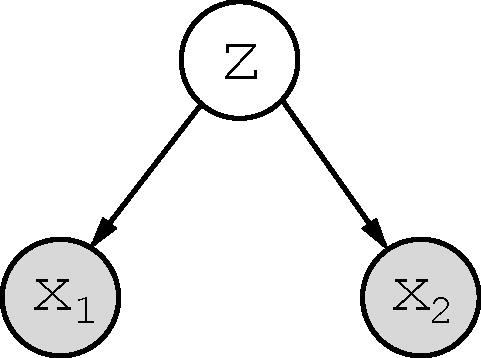
\includegraphics[width=.75\linewidth]{graph.pdf}
        \caption{}
        \label{fig:diagram:graph}
    \end{subfigure}\hspace{5mm}
    \begin{subfigure}[b]{.10\linewidth}
        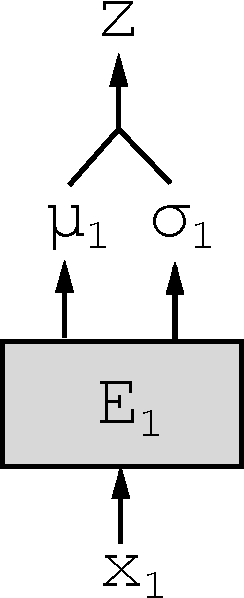
\includegraphics[width=.75\linewidth]{modelv2}
        \caption{}
        \label{fig:diagram:modelv2}
    \end{subfigure}\hspace{5mm}
    \begin{subfigure}[b]{.10\linewidth}
        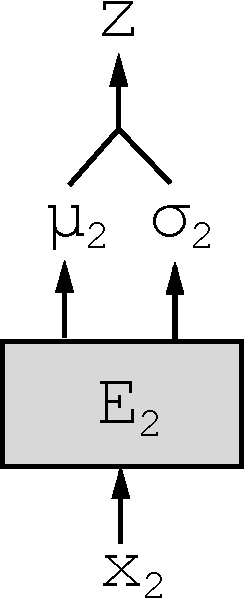
\includegraphics[width=.75\linewidth]{modelv1}
        \caption{}
        \label{fig:diagram:modelv1}
    \end{subfigure}\hspace{5mm}
    \begin{subfigure}[b]{.15\linewidth}
        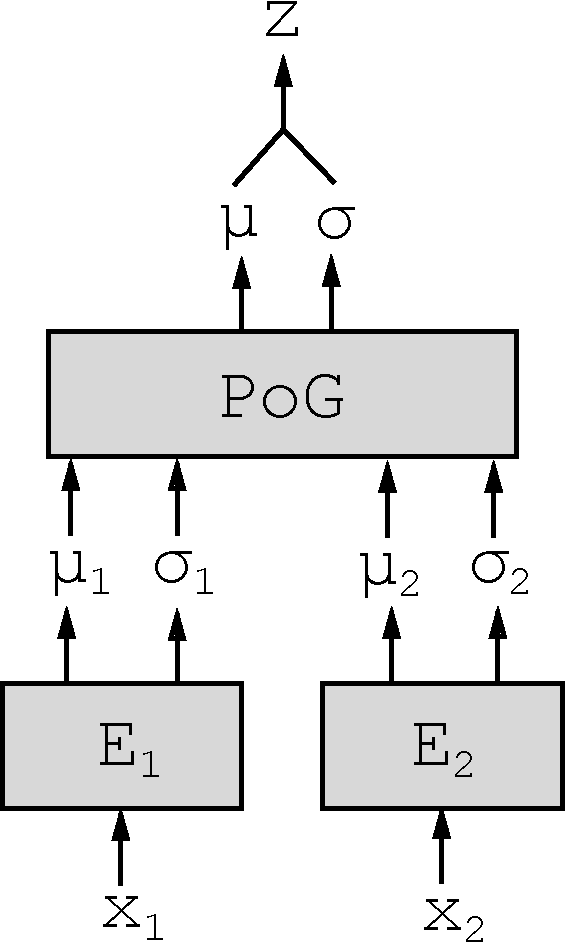
\includegraphics[width=.75\linewidth]{modelv3}
        \caption{}
        \label{fig:diagram:modelv3}
    \end{subfigure}
    \caption{(a) Graphical model of the MMVAE. Gray circles represent observed variables. The white circles represent latent variables. (b) MMVAE when modality 2 is missing. When only 1 modality is present, we ignore the PoG (product of Gaussians). (c) MMVAE when modality 1 is missing. (d) MMVAE when both modalities exist. $E_{1}$ and $E_{2}$ represent the two encoders: $q_{\phi_{x_{1}}}(z | x_{1})$ and $q_{\phi_{x_{2}}}(z | x_{2})$. Regardless if modalities are missing, we optimize the parameters of $E_{1}$ and $E_{2}$.}
    \label{fig:diagram}
\end{figure}

\subsection{Weakly-Supervised Training}
In most circumstances, paired modal data is both expensive and scarce while unimodal data, i.e. images or text is more easily available. The design of MMVAE allows for bootstrapping under sparse labels. During training, we consider input pairs of 3 types: the 1st modality alone,  the 2nd modality alone, or two separate modalities. Figure \ref{fig:diagram:modelv2}, \ref{fig:diagram:modelv1}, \ref{fig:diagram:modelv3} enumerate these three cases. In the case of a single modality, training is identical to VAE; the encoder $E_{i}(x_{i})$ returns $\mu_{i}$, $\sigma_{i}$, which is used to sample $z$ and decode. In the case of two modalities, each encoder returns $\mu_{i}$, $\sigma_{i}$, which we can combine via PoG to return the parameters of the joint Gaussian distribution. This is then used to sample $z$ and decode as in the traditional VAE. Crucially, we do not need additional loss terms or separate networks to handle unimodal and multimodal cases; the only change required is an additional PoG operation. In practice, we find that we only need a limited amount of paired multimodal examples in order to learn the cross-modal relations. 

\bibliographystyle{abbrvnat}
{\small
\linespread{1}
\bibliography{draft}
}

\end{document}